% Emacs settings: -*-mode: latex; TeX-master: "manual.tex"; -*-

\section{Chopper: The disc chopper}
\label{s:chopper}
\index{Optics!Disc chopper}

\component{Chopper}{Phillipp Bernhardt, Univ.~Erlangen (System)}{$w$, $R$, $f$, $n$, $\phi$}{IsFirst, $n_{\rm pulse}$}{}

To cut a continuous neutron beam into short pulses, or to control
the pulse shape (in time) from a pulsed source, one can use a disc
chopper (see figure~\ref{f:chopper1}). This is a fast rotating disc with the
rotating axis parallel to the neutron beam. The disk consists of neutron
absorbing materials. To form the pulses the disk has openings through which
the neutrons can pass.

Component {\bf Chopper} has $n$ openings, which are
symmetrically positioned on the disc. The direction of rotation can be controlled, 
which allows to simulate e.g. counter-rotating choppers. 
The phase (in seconds) is defined by the time 
where one slit is positioned at the top. 
The sides of the slits are pointing towards the center of the disc.
The disc is considered infinitely thin.  There is no parameter for the
size of the slits in the radial direction;
use e.g. a {\bf Slit} component in front of the chopper.

\begin{figure}[ht]
\includegraphics[width=0.8\linewidth]{figures/Chopper.eps}
\caption{Sketch of a disc chopper with geometry parameters} 
\label{f:chopper1}
\end{figure}


%Using a rectangular shaped beam with nearly the same
%size as the slit, yields an almost triangular shaped
%transmission curve (see figure~\ref{f:chopper2}).
%
%\begin{figure}[ht]
%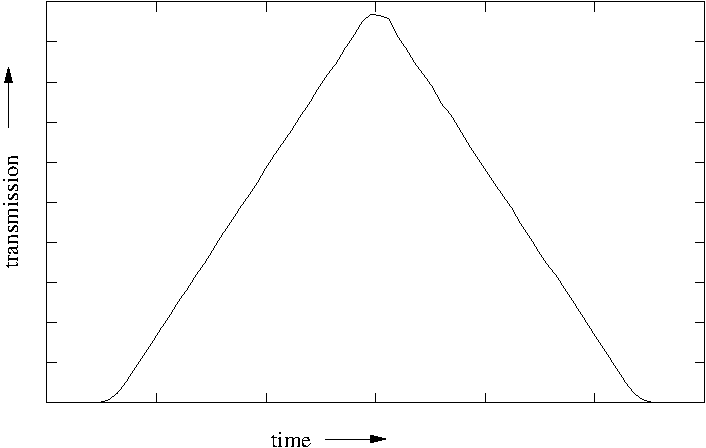
\includegraphics[width=1.0\linewidth]{figures/tracho.eps}
%\caption{example transmission curve for the disc chopper\label{f:chopper2}}
%\end{figure}

When simulating the chopping of a continuous beam,
most of the neutrons could easily be lost.
To improve efficiency, one can set the flag \verb+IsFirst+, which will
allow every neutron ray to pass the {\bf Chopper}, but modify the
time, $t$, to a (random) time at which it is possible to pass.
%This can also be used with TOF-instruments, which often
%define the starting time of the neutrons at
%the position of the first chopper.
Of course, there should be only one ``first chopper'' in
any simulation.
To simulate frame overlap from a ``first chopper'', one can specify
the number of frames to study by the parameter $n_{\rm pulse}$.
